\documentclass[12pt]{article}
\usepackage[margin=1in]{geometry}

\usepackage{float}
\usepackage{xr-hyper}
\RequirePackage[colorlinks,citecolor=blue,urlcolor=blue]{hyperref}
\usepackage{listings}
\usepackage{rotating, graphicx}
\usepackage{booktabs, natbib}

\usepackage{amsmath, enumerate, quoting, subfigure, amssymb, url}

\usepackage{color}
\newcommand{\red}[1]{\textcolor{red}{#1}}
\newcommand{\blue}[1]{\textcolor{blue}{#1}}
\newcommand{\gv}[1]{\textcolor{blue}{(GV: #1)}}
\DeclareMathOperator*{\argmin}{arg\,min}
\DeclareMathOperator*{\cov}{Cov}
\DeclareMathOperator*{\corr}{Corr}

\usepackage{xr}


% remove left indentation in itemize
\usepackage{enumitem}
\setlist[itemize]{leftmargin=*}

\usepackage{xcolor}
\newcommand{\jy}[1]{\textcolor{red}{(JY: #1)}}

% graph path
\graphicspath{{./figs/}}

\usepackage{geometry}
\geometry{vmargin={1in,1in}, hmargin={.75in, .75in}}

%\usepackage[labelfont={footnotesize,bf} , textfont=footnotesize]{caption}
%\captionsetup{labelformat=simple, labelsep=period}
%\newcommand\num{\addtocounter{equation}{1}\tag{\theequation}}
%\renewcommand{\theequation}{\arabic{equation}}
%\makeatletter
%\renewcommand\tagform@[1]{\maketag@@@ {\ignorespaces {\footnotesize{\textbf{Equation}}} #1.\unskip \@@italiccorr }}
\makeatother
\setlength{\intextsep}{10pt}
\setlength{\abovecaptionskip}{2pt}
\setlength{\belowcaptionskip}{-10pt}
\renewcommand{\textfraction}{0.10}
\renewcommand{\topfraction}{0.85}
\renewcommand{\bottomfraction}{0.85}
\renewcommand{\floatpagefraction}{0.90}

\quotingsetup{leftmargin = 0pt}

\newenvironment{comment}%
{\begin{quoting}\noindent\small\it\ignorespaces%
  }{\end{quoting}}
 \title{Points Above Replacement: A New NBA Metric to Evaluate Player Performance}
\author{
Brian Krikorian*, Jun Yan \\ \medskip 
Department of Statistics, University of Connecticut, Storrs, CT  \\  \medskip 
Students: brian.krikorian@uconn.edu* \\
Mentor: jun.yan@uconn.edu 
}

\begin{document}

\begin{titlepage}
   \begin{center}
       \vspace*{1cm}
       \Huge
       \textbf{Points Above Replacement}

       \Large
       \vspace{0.5cm}
        A New NBA Metric to Evaluate Player Performance
            
       \vspace{1.5cm}

       \textbf{Brian Krikorian}
       
       \vfill

       
\includegraphics[width=0.4\textwidth]{UCONNwordmark}

       \vfill
            
       Mentor: Jun Yan\\
       Data Science
            
       \vspace{0.8cm}
     
       
\includegraphics[width=0.4\textwidth]{UCONNoakleaf}
         
        \Large    
       Department of Statistics\\
       University of Connecticut\\
       Storrs, CT\\
            
   \end{center}
\end{titlepage}
% Abstracts are required.
\section*{Abstract}
In attempting to predict the score of an NBA game, players who are 
injured, suspended, or for any other 
reason not playing have a significant impact on said prediction. Baseball 
uses a statistic called Wins Above 
Replacement, or WAR, to tell how many wins a team would gain or lose if 
they replaced a certain player 
with one who is league average. The goal of this paper is to create a 
similar statistic, called Points Above 
Replacement, or PAR, that uses statistics from throughout the season to 
predict how many points a team 
gains or loses by missing a certain player, and thus having to replace him 
with one who is ``league 
average''. The statistic is standardized and adjusted by both position and 
value to a player's given team. 
The model roughly follows the calculation of WAR in baseball, assigning 
values to points created on offense 
and defense, as well as a positional and team adjustment. A comparison 
with the created metric along with 
other well-known advanced player metrics is done via a multiple 
regression.

% Keywords are required.
\section*{Keywords} 
Analytics; Basketball; Player Value; Sports Data; Statistics; 
\vspace{.12 in}
% Start the main part of the manuscript here.
% Comment out section headings if inappropriate to your discipline.
% If you add additional section or subsection headings, use an asterisk * to avoid numbering. 

\section{Introduction}
%Why is this important/interesting? What has been done before on this topic? (Literature Review) What am I introducing that is new? 
There exists many prediction models for NBA basketball, many with the 
purpose of anticipating the final 
score of a given game. However, the majority of these models use team 
average statistics to base their 
decisions. However, 
teams rosters can change every night, and do often. When star players 
are ruled out, players of lower 
quality take their minutes, and are expected to perform at a lower level. 
When lower level players do not 
play in a given game, star players are expected to play more minutes, 
which most likely will cause a slight 
uptick in performance. This reasoning is the cause for the creation of the 
new metric, PAR. PAR is based on the WAR statistic in baseball, which 
seeks to show player value based on average level. Many changes are 
constantly made to the statistic, however, and it is very subjective. 
\citet{Baumer} talks about how openWAR was concerned with issues of 
how WAR was previously calculated, such as accounting for uncertainty 
and reproductivity. Similarly, the measure of PAR seeks to add on to 
existing metrics by accounting for importance to a team, importance by 
position, and adjusting for amount of playing time. Points Above 
Replacement is a measure of how many points a team will gain or lose if 
a certain player does not play. 
The metric is created based on the last completed season, the 2020-2021 
season, which was cut to 72 games, as opposed to 82, due to 
the COVID-19 pandemic.

This idea of Points Above Replacement is prefaced by many different 
statistical analyses that have been done over the years. \citet{Dehesa} 
discusses the different factors that influence player performance, and 
identifies different players' profiles in order to better analyze their 
contributions to their team. Similarly, PAR is mainly concerned with a 
player's value to the team they are currently on, rather than a function of 
the entire NBA, so that individual games can be predicted more 
accurately, and also so that individual teams can analyze the value of 
their roster, which is similar to the goal of the cited paper, and a part of 
where the influence was drawn.

\citet{Fearnhead} also tries to find a way to estimate NBA player ability. 
The analysis is based on splitting player value into offensive and 
defensive categories, then combining the two to get a total value. WAR is 
calculated very similarly, in that it assigns a value to all aspects of 
baseball, and then combines them \citep{BaseballWAR}. PAR also 
assumes this method to create the metric, which will be discussed later. 
Another aspect of this analysis that PAR takes on is centering the data, so 
that the league average is 0, and all other data can be based around that. 
A key difference is that while this paper does break up the analysis by 
position, it only recognizes 3 different positions, while PAR looks at all 5 
individual positions in the NBA.

No similar papers where a new NBA statistic to analyze individual points 
that a player adds to his team were found, but pieces of other NBA 
analytics were very influential in the creation of PAR. Similar to how 
openWAR sought to fix the typical WAR statistic, PAR seeks to stand out 
from other accepted advanced metrics, such as BPM and PER. 
\citet{Hamalian} talks about the flaws that exist in PER, such as the lack 
of centering in the data, making the league average actually vary per 
season. The cited article also talks about how the pace statistic in PER 
ultimately does not do anything. Thus, PAR takes many of the same 
box-score 
statistics that PAR does, but seeks to center its data to form a 
season-by-season league average, and attributes a player's value to his 
team's total points and total minutes, rather than accounting for the pace 
of the team. There are similarities with PER that this article still believes 
are not efficient, and those shortcomings will be discussed further in later 
sections.

One of the main adjustments in PAR that occurs is that of a positional 
adjustment. Different positions have different requirements, so box score 
statistics need more analysis than meets the eye to really show a player's 
value. \citet{Piette} makes a point of this in the analysis of field goal 
percentage based on distance from the basket. Adjusting by positional 
need is a key aspect of PAR that was inspired by the metrics in the cited 
paper. Players in the NBA all have different skillsets, and different 
positions call for these specific skillsets in order for a team to be 
successful as a unit, which is a key point in the cited paper, as well as in 
PAR.

As previously stated, there were no other papers found in which a new 
NBA metric was attempted to be created, so the question is that of what 
PAR can add to previously accepted statistics.
Position and team adjustments 
allow for a player's value to his 
specific team to be measured, giving a better expectation for their 
presence or absence. This is similar to how WAR is calculated, which 
takes into account a positional and league adjustment 
\citep{BaseballWAR}. Adjusting to a 
position allows one to analyze a player based on what his position 
requires. The team adjustment is a function of how 
many minutes a player played 
throughout the entire season, and how many of their team's total points 
were scored by them. If a player 
plays a majority of his team's minutes, and scores a relatively high 
percentage of his team's points, he will 
be more valuable to his team, and his team will be hurt more by his 
absence in a game. The idea of how much an individual team will value 
an individual player is the key unique factor in PAR that causes it to stand 
out.


\section{Data}
% Include basic graphics here?
All basic and advanced statistics from the 2020-2021 season were 
collected from the Basketball Reference 
website, as well as each team's total points throughout the course of the 
season \citep{BasketballReference}. From the basic statistics, 4 metrics 
were 
created in order to calculate PAR. 
Offensive Points is a function of how many points a player will create on 
offense. While the coefficients vary 
by position, the statistics used are effective field goal percentage, three 
point percentage, free throw 
percentage, offensive rebounds, assists, points, and turnovers. Similarly, 
Defensive Points is a function of how many points a player helps prevent 
while his team is on defense. The coefficients also vary by position, 
but this metric is based on defensive rebounds, total rebounds, steals, 
blocks, and personal fouls. 

The Positional Adjustment metric creates a coefficient of how valuable a 
player is to their individual team, and is 
based on how many minutes a player plays relative to their team, as well 
as how many points they score 
relative to their teams total points. The last statistic created is Points Per 
Win, which is based on the 
average amount of points a player will create in a game. This function is 
based on the sum of Offensive and 
Defensive Points, and is scaled to incorporate the total number of games, 
minutes, and players in a season. 
This statistic is very similarly calculated to Runs Per Win in the WAR 
statistic. Given that over the course of 
a 72 game season, all teams will play each other at least once, we 
assume a relatively equal distribution in 
terms of strength of schedule. 

Advanced statistics for each player were also collected in order to perform 
a 
regression, to see how PAR compares with known and accepted metrics. 
Value Over Replacement Player, 
also known as VORP, was one of the metrics used, and is calculated with 
the help of Box Score Plus 
Minus, also known as BPM. These statistics also help give a relative 
estimate of a player's value compared 
to that of an average player, but they translate the statistic to a league 
average team as well. PAR does not 
do this, because it is concerned with how valuable a player is to his 
specific team, not throughout the entire 
league. If a player switched teams, his PAR value would most likely 
change, as his importance to one team 
may be more or less than it would to another. For simplicity, the team that 
a player played his most games 
on was taken into consideration for this metric. 

Similarities to BPM, and therefore VORP, can be explained by many 
different factors. BPM centers data so that the league average is 0, and 
creates coefficients for factors based on a player's position and offensive 
role. While PAR is not concerned with offensive role, it does take into 
account position, and assumes that position, for the most part, is 
correlated with offensive role. Intentional usage of only universally 
available statistics allow for easy calculation as well as easy 
understanding for audiences. The key difference is that of playing time not 
being a factor in BPM and VORP, which is obviously a key factor in PAR 
\citep{BasketballReferenceBPM}.

Other statistics used include Player Efficiency Rating, a 
per-minute rating of player performance, and Win Shares, which 
estimates the number of wins a player creates 
for his team throughout the season. Due to all of these metrics' relative 
similarity to PAR, it is suggested 
that if they are highly correlated with PAR, it is a successful metric. 
However, we expect some differentiation 
between the metrics, as they all vary slightly in what they attempt to 
convey. The relative correlation 
between all these statistics shows that PAR is related to other advanced 
metrics analyzing player efficiency, 
but also that it introduces something new in basketball statistics.



\section{Methods}
% Should dive more in depth about how everything was obtained, calculated, etc.

The basic method for calculating the PAR method was based on how 
WAR is calculated in baseball, but 
also took influences from other advanced basketball statistics. WAR is 
based on Offensive and Defensive 
Runs, which are calculated subjectively via attributes of the game such as 
hitting, base running, fielding, 
and so forth \citep{BaseballWAR}. The subjectivity is in the coefficients 
chosen to scale 
statistics which impact Offensive and 
Defensive Runs. Thus, there are actually an infinite different kinds of WAR 
in baseball, depending on which 
method of calculating Offensive and Defensive Runs is used. Similarly, 
PAR is created by calculating 
Offensive and Defensive Points statistics, to analyze how many points a 
player adds for his team, and how 
many he prevents the other team from scoring. 

Using the basic offensive 
statistics of Effective Field Goal 
Percentage, Three Point Percentage, Free Throw Percentage, Offensive 
Rebounds, Assists, Points, and 
Turnovers, we assign a coefficient to them based on how important they 
are for a given position. Point 
guards are expected to pass more than centers, and a point guard's 
passing ability has more value to his 
team than a center, so more weight is placed on that statistic for point 
guards. This goes for all positions, 
and a coefficient matrix of a constant scale is created. That is to say, 
assists have a coefficient from point 
guards, shooting guards, small forwards, power forwards, and centers, 
respectively, of 4, 3.5, 3, 2.5, and 2. 

The coefficient by position method is one similar to that of Box Plus 
Minus, another advanced NBA metric \citep{BasketballReferenceBPM}. 
The position a player was assigned for the calculation was the position 
where he played the most minutes 
throughout the 2020-2021 season. This coefficient method gives a clean 
scaling into the calculation of 
Offensive Points. Some statistics, such as Points and Effective Field Goal 
Percentage, are equally 
important, regardless of the position of a given player. Thus, these 
statistics have a constant coefficient that 
does not change. Once all coefficients were applied to all statistics, the 
sum was taken to give Offensive 
Points. 

The exact same method was applied to the Defensive Points 
calculation, but used the basic 
defensive statistics of Defensive Rebounds, Total Rebounds, Steals, 
Blocks, and Personal Fouls. As 
turnovers and personal fouls are not desirable amongst players, the 
coefficients for these statistics is 
negative, which allows for a scale of not only the good a player does, but 
also what they do poorly. This 
coefficient method is similar to the Positional Adjustment metric applied in 
WAR calculation, which seeks to 
adjust a player's importance based on what is expected of their position.

 
The coefficients for each position are listed in Table~
\ref{tab:Coefficientstable}. Coefficients are subjective, but were changed 
to have a constant scale by position, and create a PAR scale that lined up 
closely with other advanced metrics. This coefficient matrix could be 
looked at as an optimization problem, where coefficients by position are 
changed to achieve as high of a correlation with other advanced metrics 
as possible. However, a constant scale by position and a relatively high 
correlation to other metrics shows uniqueness in the statistic but also 
validity.

\begin{table}[H]
  \caption{Coefficients for Each Statistic in Offensive and Defensive Points}
  \label{tab:Coefficientstable}
\centering
\begin{tabular}[t]{lcccccc}
  \toprule
  Statistic & Point & Shooting & Small & Power  & Center\\
  & Guard & Guard & Forward & Forward & \\
  \midrule
 Effective FG Percentage & 200 & 200 & 200 & 200 & 200\\
 3 Point Percentage & 300 & 275 & 250 & 225 & 200\\
 Free Throw Percentage & 100 & 90 & 80 & 70 & 60\\
 Offensive Rebounds & 1 & 1.5 & 2 & 2.5 & 3\\
 Assists & 4 & 3.5 & 3 & 2.5 & 2\\
 Points & 2 & 2 & 2 & 2 & 2\\
 Turnovers & $-5$ & $-4.5$ & $-4$ & $-3.5$ & $-3$\\
 Defensive Rebounds & 2 & 2.5 & 3 & 3.5 & 4\\
 Total Rebounds & 3 & 3.25 & 3.5 & 3.75 & 4\\
 Steals & 5 & 4.5 & 4 & 3.5 & 3\\
 Blocks & 3 & 3.5 & 4 & 4.5 & 5\\
 Personal Fouls & $-3$ & $-3$ & $-3$ & $-3$ & $-3$\\
  \bottomrule
\end{tabular}
\end{table}

The next step was creating a Team Adjustment statistic. As stated before, 
the PAR metric seeks to 
anticipate how valuable a player is to their given team, rather than as an 
average of the entire league. This 
gives more of an insight of how a team will fare without a certain player. 
We expect this statistic to change if 
a player were to switch teams. This is similar to the League Adjustment in 
WAR calculation, where a 
player's value is adjusted based on whether he plays in the American 
League or the National League. The 
Eastern and Western Conferences in the NBA have much less disparity 
compared to the MLB, and each 
conference plays each other much more frequently, so we instead change 
this to adjust a player's value to 
his specific team. The team assigned to a given player was the team 
where he played the most games 
during the 2020-2021 season. If a player had played an even amount of 
games for 2 separate teams, the 
team the player had played the most minutes for was assigned as his 
team. 

The Team Adjustment statistic 
is then calculated by taking the total minutes a player was on the court 
during the entire season, and diving 
it by a constant of 3,456 (the maximum number of minutes a player could 
have played during the shortened 
season, 48 minutes per game multiplied by 72 games). Then, the 
percentage of points a player scored for 
his team (player's total points divided by team's total points throughout the 
season) was calculated, and the 
two results were multiplied together. As a player cannot play 100 percent 
of his team's minutes, or score 
100 percent of his team's points, the result is a number between 0 and 1. 

A similar adjustment is also used 
in the calculation of Box Plus Minus, which is a key factor in calculating 
Value Over Replacement Player, 
two of the advanced metrics PAR will be compared against. The goal of 
this adjustment is to give less of a 
penalty to players who play a majority of their team's minutes, and score a 
majority of their team's points. 
This helps truly elite players stand out amongst the pack, as well as 
players who may not be the best of the 
best, but matter more to their team specifically than in the grand scheme 
of things.

Lastly, WAR implements a Runs Per Win statistic, which gives a basic 
idea of how many runs are needed 
for a win in the MLB. Similarly, a Points Per Win statistic is created for the 
NBA, which allows a scaling 
down of the PAR statistic. We calculate this via the combined Offensive 
and Defensive Points statistic for a 
player divided by the number of minutes he played, then adding 2,160 (72 
games per season times 30 
teams in the NBA, thus, the total number of chances to win throughout the 
season). This gives a basic 
metric of a players points created as a function of how many minutes he 
played, and allows us to even the 
metric out a bit more from star players to role players. This statistic serves 
as the denominator of our PAR 
calculation.

Once all supporting statistics of PAR have been created, all that is left to 
do is combine them to achieve our PAR values for each player in the 
NBA. The formula for PAR is listed below.

\begin{equation}
 \label{eq:PAR}
  \frac{(\text{Offensive Points} + \text{Defensive Points}) \times \text{Team Adjustment}}
  {\text{Points Per Win}}.
\end{equation}

Equation~\ref{eq:PAR} gives a good idea of how many points a player 
accounts for 
during a 
game, how important that is for 
his given team, and how important it is compared to all other players. The 
last step is to standardize this 
PAR statistic, so that the mean is 0, and the standard deviation is 1. 
Logically, this helps the idea of the 
metric in the sense that a perfectly league average player should have a 
PAR of 0, and his presence or 
absence from his team neither adds nor subtracts value. Thus, we have 
created a new NBA player metric, 
Points Above Replacement, PAR. All of the calculations, multiple 
regression, and graphs were created using R \citep{R}.
 
 
\section{Results}
% Multiple Regression
% Analyze Graphs of PAR, filter by position perhaps?
% Any other tests that should be done?
First, the top 10 players in terms of PAR in the league will be analyzed. Then, the top 10 PAR values at each position will be evaluated.

\begin{table}[H]
  \caption{PAR Values from the Entire NBA}
  \label{tab:NBAtable}
\centering
\begin{tabular}[t]{lcccccc}
  \toprule
  Rank & Player & Position & Team & PAR\\
  \midrule
 1 & Nikola Jokic & C & Denver Nuggets & 7.69\\
 2 & Nikola Vucevic & C & Orlando Magic & 6.55\\
 3 & Julius Randle & PF & New York Knicks & 6.49\\
 4 & Luka Doncic & PG & Dallas Mavericks & 4.61\\
 5 & Damian Lillard & PG & Portland Trail Blazers & 4.47\\
 6 & Giannis Antetokounmpo & PF & Milwaukee Bucks & 4.21\\
 7 & Stephen Curry & PG & Golden State Warriors & 4.17\\
 8 & Russell Westbrook & PG & Washington Wizards & 4.05\\
 9 & Jayson Tatum & SF & Boston Celtics & 3.96\\
 10 & Domanatas Sabonis & PF & Indiana Pacers & 3.21\\
 \bottomrule
\end{tabular}
\end{table}

As can be seen in Table~\ref{tab:NBAtable}, one player rises above all 
others in 
both PAR and VORP. 
That player is Nikola Jokic of the 
Denver Nuggets, and this ``outlier'' makes perfect sense, and helps show 
just how dominant his MVP 
season was. Not only did Jokic average 26.4 points, 10.8 rebounds, and 
8.3 assists per game, he was 
doing it from the center position. Having a center that has the ability to 
perform in all aspects of the game, 
even those that his position does not require, proves his value to his 
team, which is why his value is so 
much higher in both the new PAR metric, and the accepted VORP metric. 
This logic applies to Nikola 
Vucevic, Julius Randle, Russell Westbrook, and Domanatas Sabonis as 
well. While they might not be 
considered the best at their position, or an extremely elite player in the 
NBA, they are very versatile players, 
that can do anything on the court, and thus they are rewarded with a high 
PAR value. This makes sense, as 
without these players, a lot of the statistics their team accumulates are 
gone, so while they may not have as 
much value in the grand scheme of the NBA, they were very much the 
most valuable players for their 
teams. Another key thing to note is that some players, such as LeBron 
James, have a lower PAR than 
expected, and this could be due to the fact that they played most 
frequently in a position that did not match 
their skill set. LeBron James played primarily as a point guard, but his 
skillset matches that of a small 
forward or power forward. Thus, his strengths are not adequately 
measured, as he is essentially being 
played ``out of position''.

\begin{table}[H]
  \caption{PAR Values from all Point Guards}
  \label{tab:PGtable}
\centering
\begin{tabular}[t]{lcccccc}
  \toprule
  Rank & Player & Team & PAR\\
  \midrule
 1 & Luka Doncic & Dallas Mavericks & 4.61\\
 2 & Damian Lillard & Portland Trail Blazers & 4.47\\
 3 & Stephen Curry & Golden State Warriors & 4.17\\
 4 & Russell Westbrook & Washington Wizards & 4.05\\
 5 & Trae Young & Atlanta Hawks & 2.69\\
 6 & De'Aaron Fox & Sacramento Kings & 1.94\\
 7 & Chris Paul & Phoenix Suns & 1.93\\
 8 & Kyrie Irving & Brooklyn Nets & 1.74\\
 9 & Dejounte Murray & San Antonio Spurs & 1.64\\
 10 & Ja Morant & Memphis Grizzlies & 1.45\\
  \bottomrule
\end{tabular}
\end{table}

\begin{table}[H]
  \caption{PAR Values from all Shooting Guards}
  \label{tab:SGtable}
\centering
\begin{tabular}[t]{lcccccc}
  \toprule
  Rank & Player & Team & PAR\\
  \midrule
 1 & Bradley Beal & Washington Wizards & 3.17\\
 2 & Devin Booker & Phoenix Suns & 2.74\\
 3 & Terry Rozier & Charlotte Hornets & 2.59\\
 4 & Zach Lavine & Chicago Bulls & 2.29\\
 5 & RJ Barrett & New York Knicks & 2.28\\
 6 & Anthony Edwards & Minnesota Timberwolves & 2.22\\
 7 & Jaylen Brown & Boston Celtics & 1.87\\
 8 & Collin Sexton & Cleveland Cavaliers & 1.85\\
 9 & Buddy Hield & Sacramento Kings & 1.72\\
 10 & Norman Powell & Toronto Raptors & 1.37\\
  \bottomrule
\end{tabular}
\end{table}

\begin{table}[H]
  \caption{PAR Values from all Small Forwards}
  \label{tab:SFtable}
\centering
\begin{tabular}[t]{lcccccc}
  \toprule
  Rank & Player & Team & PAR\\
  \midrule
 1 & Jayson Tatum & Boston Celtics & 3.96\\
 2 & Khris Middleton & Milwaukee Bucks & 2.39\\
 3 & Brandon Ingram & New Orleans Pelicans & 2.13\\
 4 & Kawhi Leonard & Los Angeles Clippers & 1.58\\
 5 & Paul George & Los Angeles Clippers & 1.44\\
 6 & Michael Porter Jr. & Denver Nuggets & 1.42\\
 7 & Jimmy Butler & Miami Heat & 1.41\\
 8 & Bojan Bogdonavic & Utah Jazz & 1.35\\
 9 & Mikal Bridges & Phoenix Suns & 1.19\\
 10 & Jerami Grant & Detroit Pistons & 1.14\\
  \bottomrule
\end{tabular}
\end{table}

\begin{table}[H]
  \caption{PAR Values from all Power Forwards}
  \label{tab:PFtable}
\centering
\begin{tabular}[t]{lcccccc}
  \toprule
  Rank & Player & Team & PAR\\
  \midrule
 1 & Julius Randle & New York Knicks & 6.49\\
 2 & Giannis Antetokounmpo & Milwaukee Bucks & 4.21\\
 3 & Domanatas Sabonis & Indiana Pacers & 3.21\\
 4 & Zion Williamson & New Orleans Pelicans & 3.07\\
 5 & Andrew Wiggins & Golden State Warriors & 2.26\\
 6 & Demar Derozan & San Antonio Spurs & 1.88\\
 7 & Tobias Harris & Philadelphia 76ers & 1.87\\
 8 & Pascal Siakam & Toronto Raptors & 1.72\\
 9 & John Collins & Atlanta Hawks & 1.35\\
 10 & Harrison Barnes & Sacramento Kings & 1.11\\
  \bottomrule
\end{tabular}
\end{table}

\begin{table}[H]
  \caption{PAR Values from all Centers}
  \label{tab:Ctable}
\centering
\begin{tabular}[t]{lcccccc}
  \toprule
  Rank & Player & Team & PAR\\
  \midrule
 1 & Nikola Jokic & Denver Nuggets & 7.69\\
 2 & Nikola Vucevic & Orlando Magic & 6.55\\
 3 & Rudy Gobert & Utah Jazz & 3.10\\
 4 & Bam Adebayo & Miami Heat & 2.78\\
 5 & Joel Embiid & Philadelphia 76ers & 2.26\\
 6 & Clint Capela & Atlanta Hawks & 2.25\\
 7 & DeAndre Ayton & Phoenix Suns & 2.11\\
 8 & Jonas Valanciunas & Memphis Grizzlies & 1.98\\
 9 & Karl-Anthony Towns & Minnesota Timberwolves & 1.82\\
 10 & Kelly Olynyk & Miami Heat & 1.39\\
  \bottomrule
\end{tabular}
\end{table}

PAR will also be compared with the 4 accepted advanced metrics that 
were used as regressors in the 
multiple regression on PAR. These include Player Efficiency Rating, Win 
Shares, Box Plus Minus, and 
Value Over Replacement Player.

\begin{figure}[H]
  \centering
  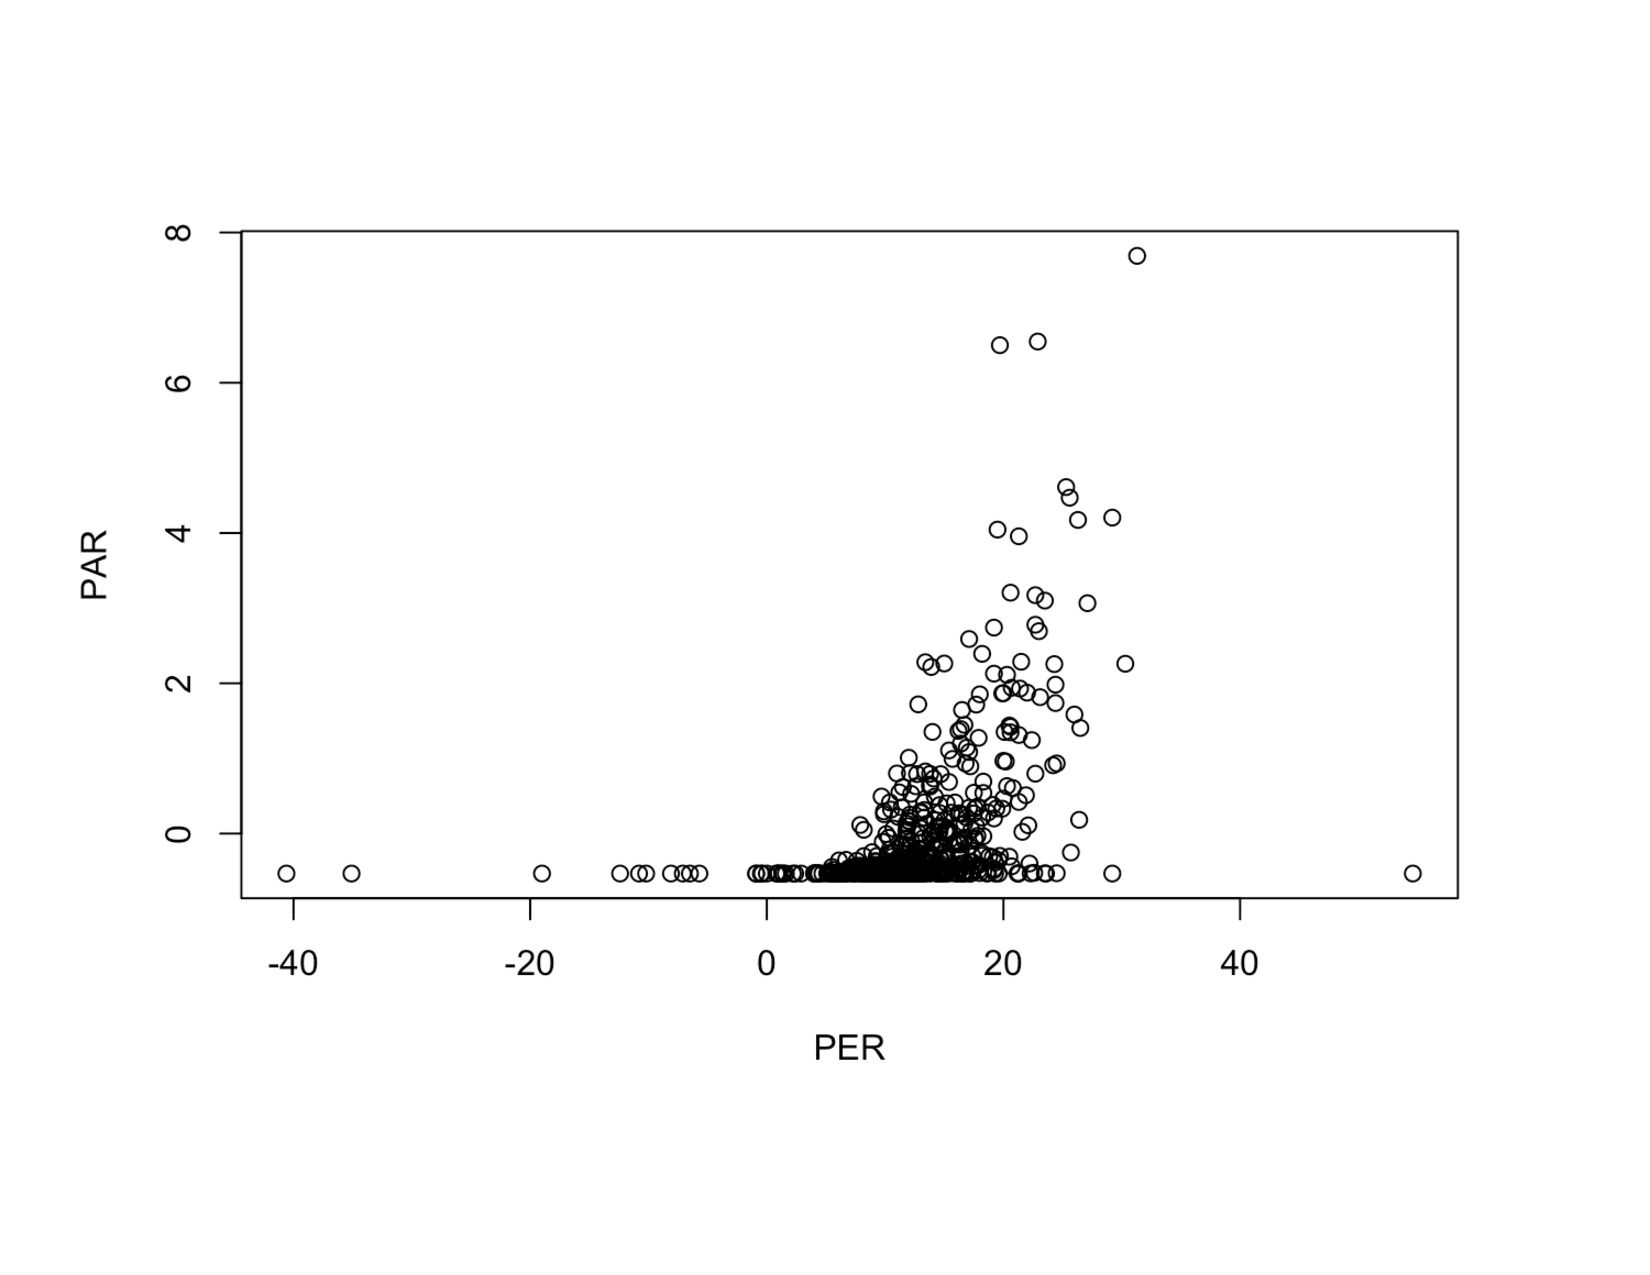
\includegraphics[width=\textwidth]{PERvsPAR}
  \caption{Player Efficiency Ratings (x) vs. Points Above Replacement (y)}
  \label{fig:Fig1}
\end{figure}

\begin{figure}[H]
  \centering
  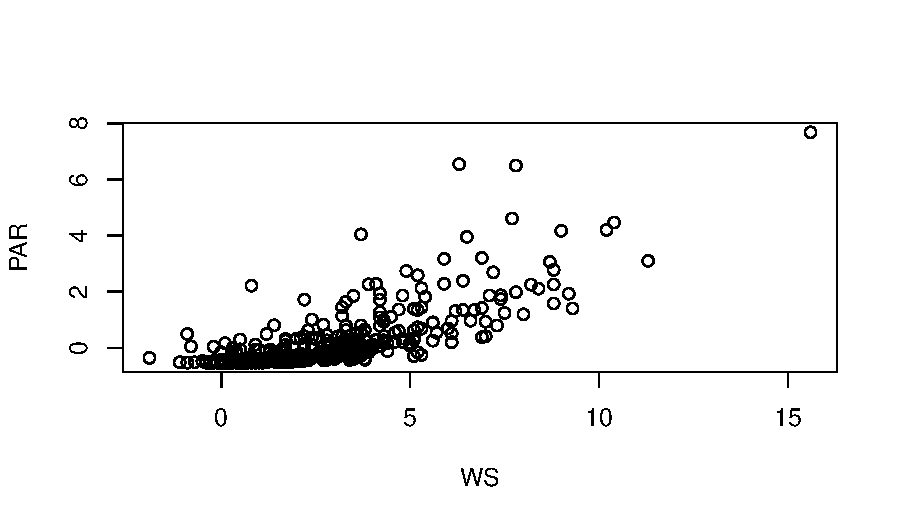
\includegraphics[width=\textwidth]{WSvsPAR}
  \caption{Win Shares (x) vs. Points Above Replacement (y)}
  \label{fig:Fig2}
\end{figure}

\begin{figure}[H]
  \centering
  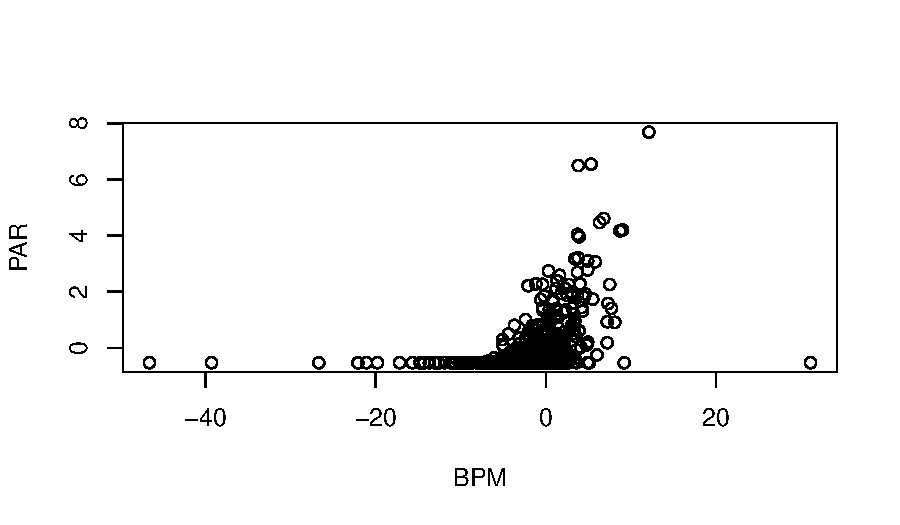
\includegraphics[width=\textwidth]{BPMvsPAR}
  \caption{Box Plus Minus (x) vs. Points Above Replacement (y)}
  \label{fig:Fig3}
\end{figure}

\begin{figure}[H]
  \centering
  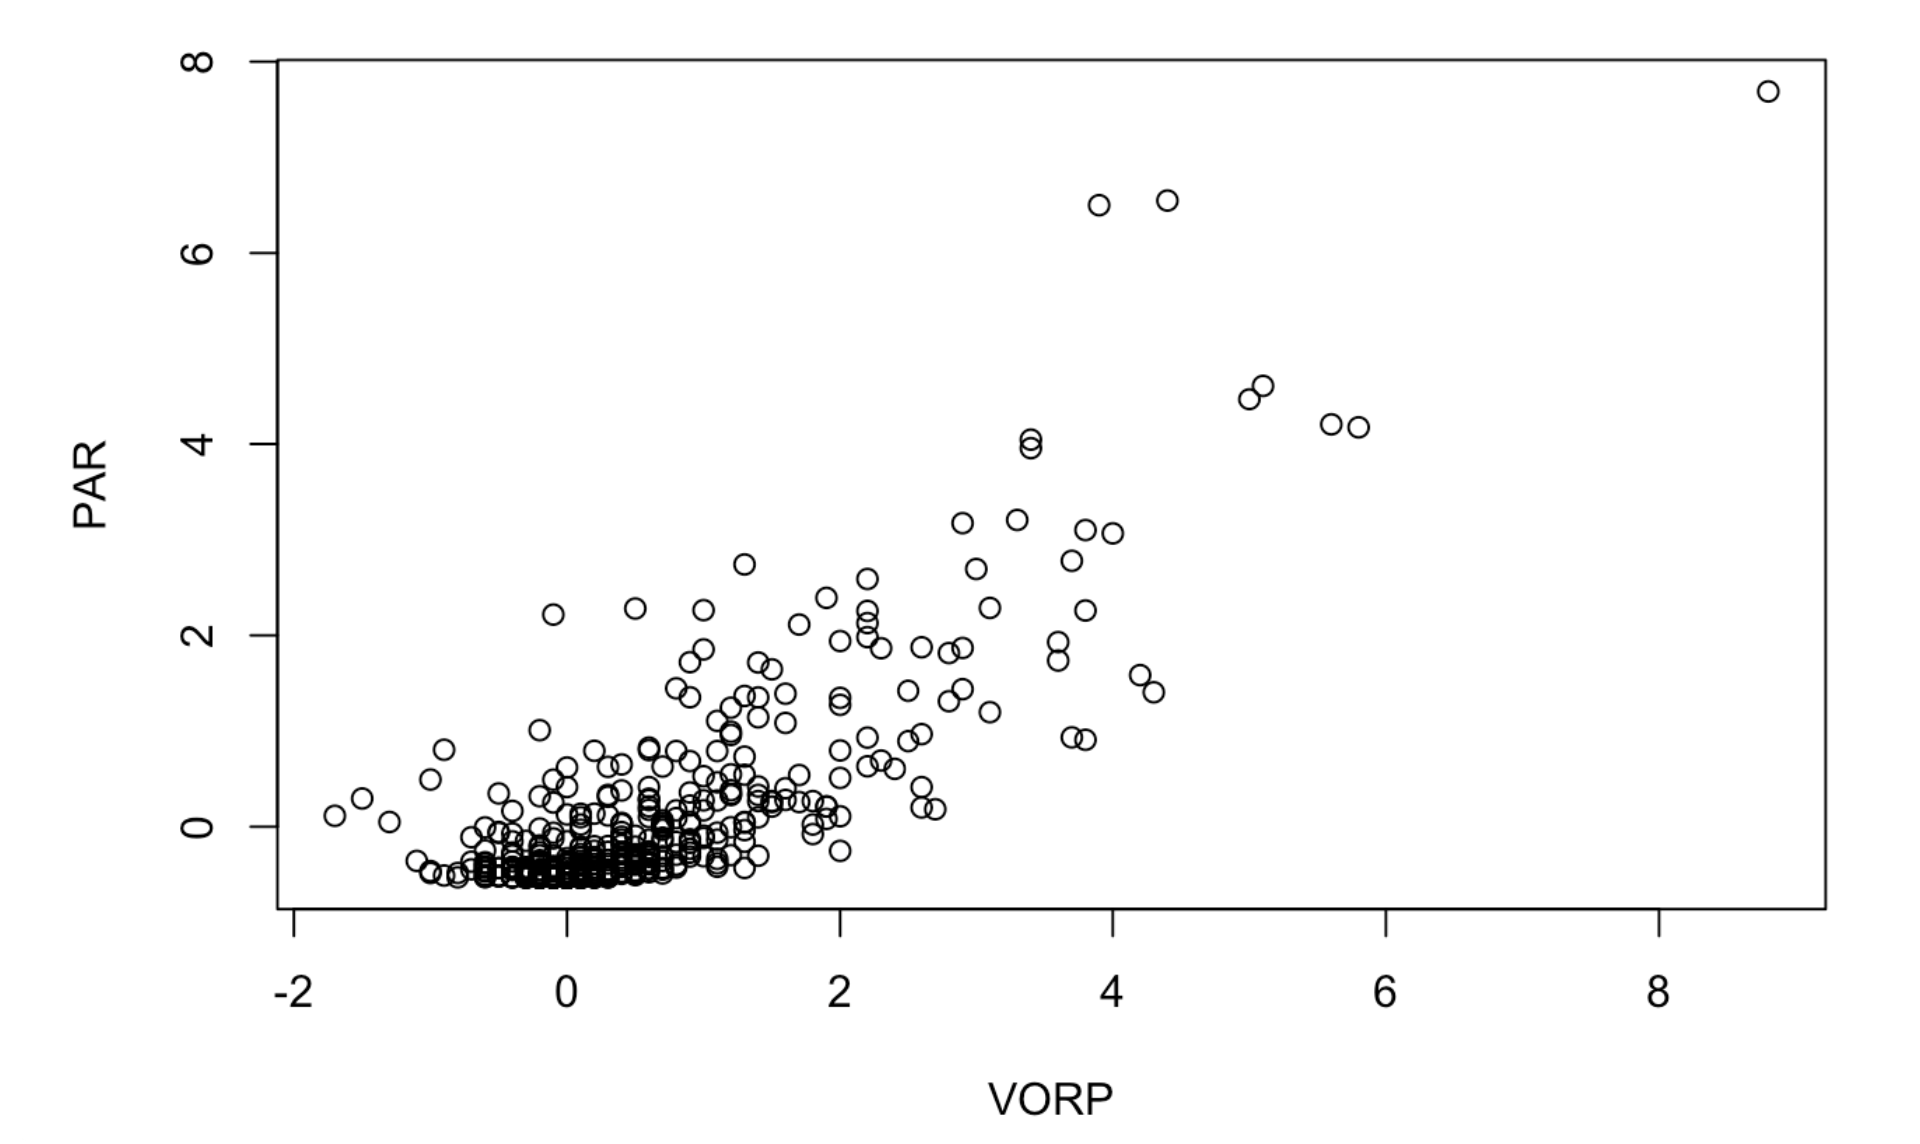
\includegraphics[width=\textwidth]{VORPvsPAR}
  \caption{Value Over Replacement Player (x) vs. Points Above Replacement (y)}
  \label{fig:Fig4}
\end{figure}

It can be seen in Figure~\ref{fig:Fig2} that the graphs of PAR and Win 
Shares, as 
well as PAR 
and Value Over Replacement Player in Figure~\ref{fig:Fig4}
fit nicely, with a relatively positive and linear correlation. However, the 
graphs of PAR and Box Plus Minus in. Figure~\ref{fig:Fig3}, 
as well as PAR and Player Efficiency Rating in Figure~\ref{fig:Fig1} 
appear to 
have less of a 
linear distribution. This can be 
attributed to the scaling methods of each statistic. Since Win Shares and 
Value Over Replacement Player 
follow a similar scale, with a minimum slightly below 0, and a maximum 
somewhere in the range of 10, the 
scales match, and each player's value of each metric fits similarly enough 
to form a linear distribution in both Figure~\ref{fig:Fig2} and 
Figure~\ref{fig:Fig4}. 
However, Box Plus Minus ranges from -40 to above 20, so we see the 
graph of Figure~\ref{fig:Fig3} centered around 0, where the 
majority of players fall, and going almost straight upwards based on their 
PAR value. Player Efficiency 
Rating has a similar scale, so a similar effect is shown in 
Figure~\ref{fig:Fig1}. In 
order to see 
how Points Above Replacement fits 
in terms of all of these accepted metrics, a multiple regression will be run, 
with the 4 accepted metrics as 
regressors, and with PAR as the independent variable.

\begin{table}[H]
  \caption{Multiple Regression on PAR}
  \label{tab:MultipleRegression}
\centering
\begin{tabular}[t]{lcccccc}
  \toprule
  Variable &  Estimate & Standard Error & P-Value\\
  \midrule
Intercept & $-1.009$  & 0.145 & $9.44 \times 10^{-12}$\\
PER & 0.030 & 0.009 & 0.002\\
WS & 0.121 & 0.024 & $4.75 \times 10^{-7}$\\
BPM & $-0.057$ & 0.013 & $1.27 \times 10^{-5}$\\
VORP & 0.559 & 0.049 & Less Than $2 \times 10^{-16}$\\
  \bottomrule
\end{tabular}
\end{table}

In Table~\ref{tab:MultipleRegression} an adjusted R-squared value of 
0.6974 is shown, along with an SER of 0.5501. The adjusted R-squared
statistic is key, as it shows that 69.74 percent of variation 
in PAR can be explained by these other 4 accepted metrics. This shows a 
clear correlation between PAR 
and the metrics, but also shows that PAR has something unique to offer.




\section{Discussion}
% Analyzing entire study, show how you can use PAR now, did it achieve the overall goal I was looking for?
% Talk about drawbacks, what could be improved, etc.
% Talk about how it is in agreement with existing measures
Ultimately, the goal of this statistic is to allow a reader to gauge a player's 
value to his team based on a 
league average player. As previously stated, the metric is adjusted so that 
a league average player has a 
PAR value of 0. Based on all other players' PAR values, we can create a 
sort of ``legend'', a rough guideline 
for what a player's role will be based on the threshold his PAR value falls 
under.

\begin{table}[H]
  \caption{PAR Legend}
  \label{tab:PARLegend}
\centering
\begin{tabular}[t]{lcccccc}
  \toprule
  Role &  PAR\\
  \midrule
Benchwarmer & Less than $-0.43$\\
Role Player & $-0.43$ to 0.08\\
Starter & 0.08 to 1.09\\
All-Star & 1.09 to 1.94\\
Superstar & Greater than 1.94\\
  \bottomrule
\end{tabular}
\end{table}

This legend in Table~\ref{tab:PARLegend} was calculated based on a 
quantile 
calculation of all PAR 
data. It is not an even distribution, as 
it is assumed that there are many more benchwarmers in the NBA than 
there are superstars. Thus, 
benchwarmers are defined as the bottom 50 percent of the league, as an 
NBA roster of about 15 players 
will only give 7 or 8 players significant minutes. Players between the 50th 
and 75th percentile are defined 
as role players, as they get significant minutes, but do not make an impact 
enough to be considered a solid 
starter. This is where  a `league average'' player is expected to fall, as 0 is 
contained in this part of the 
legend, and 0 represents a league average player via this metric. Next, 
the 75th to 90th percentile are 
defined as starters, because only 5 players can start a game, and, more 
often than not, a team only has 3 
or 4 players who are guaranteed starters. The 90th to 95th percentiles 
represent all-stars, as that is clearly a 
very prestigious area to be a part of. Lastly, it is assumed that only the top 
5 percent of players in the 
league can be deemed ``superstars'', so they comprise the 95th to 100th 
percentile of the NBA. By this 
method, it is felt that a more realistic legend for PAR has been created as 
opposed to just breaking up the 
data evenly into 5 groups.


\bibliographystyle{chicago}
\bibliography{citations}

%\section*{Acknowledgements}
%The authors thank the University of Connecticut and the UConn Department of Statistics.



%Note correct LaTeX quotations above. Do not use the " symbol, but rather double ` followed by double '



% The About the Student Author section is NOT optional.  Write a paragraph about the student; see previous journal editions for examples.
% If there is more than one student author, you must move the comment below.
\section*{About the Student Author}
Brian Krikorian plans to graduate in May 2022 from the University of 
Connecticut, with a Bachelor's of Science in Data Science, and a minor in 
Computer Science.

% The Press Summary section is NOT optional.  Write a paragraph describing the paper in a manner suitable for the press; see previous journal editions for examples.

%\section*{Press Summary}

\end{document}